\subsection{Class Diagram}

%\subsubsection{Trainee}
%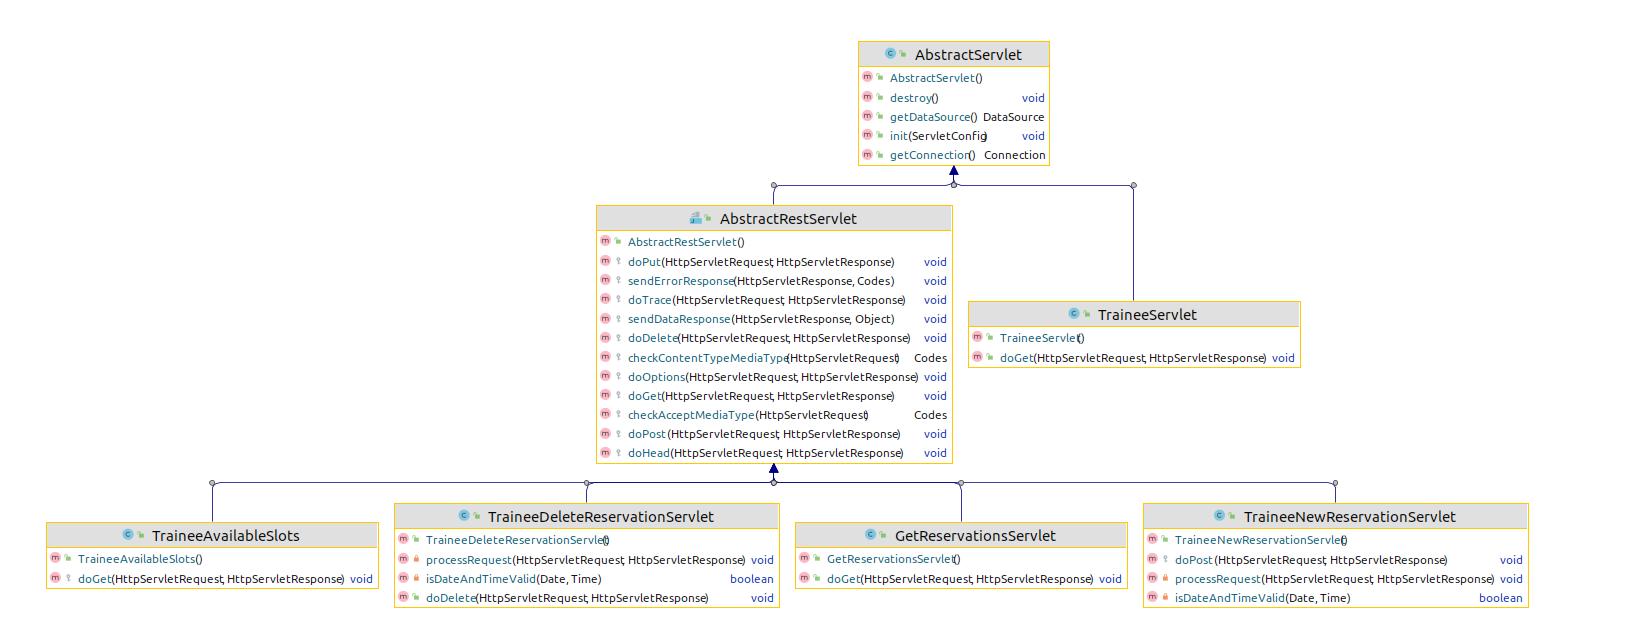
\includegraphics[width=\columnwidth]{resources/ClassDiagram_traineeServlets.png}

%Here, there is the Class Diagram that depicts the Trainee Resource (Dao omitted due to space). As we can see there are 5 main servlets for this resource : TraineeAvailableSlotsServlet, TraineeDeleteReservationServlet, GetReservationServlet, TraineeNewReservationServlet, TraineeServlet. The first four servlets are used to manage the main operation that a trainee can do, while the other one manage the Trainee page generally.

%\subsubsection{Trainer}
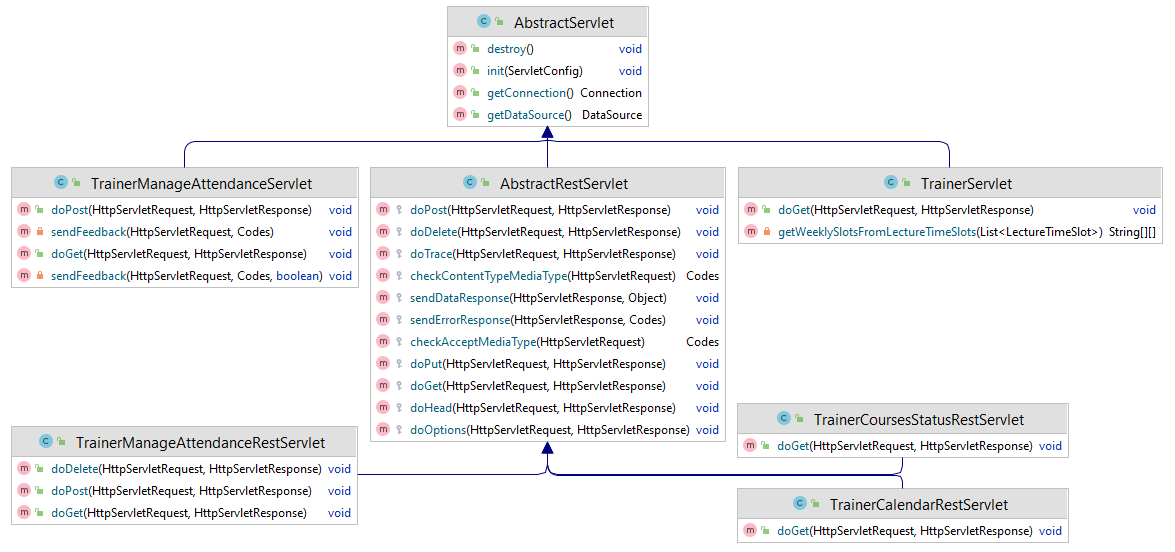
\includegraphics[width=\columnwidth]{resources/ClassDiagram_trainerServlets.png}
The Class Diagram above depicts the Trainer Resource. There are 5 main servlets for this resource : TrainerManageAttendanceRestServlet, TrainerManageAttendanceServlet, TrainerCoursesStatusRestServlet, TrainerCalendarRestServlet, and TrainerServlet. The first Servlet is used to manage attendance through REST API calls meanwhile the second one does the same thing via a JSP page. TrainerServlet returns trainer's courses with his current weekly schedule. TrainerCoursesStatusRestServlet and TrainerCalendarRestServlet does the same thing but via REST API calls.
